\section{Results}
\subsection{Low Noise Amplifier}
Fig. ~\ref{fig:s11} shows the S11 parameters of the LNA, which indicates the input matching quality. The minimum input matching is -21 dB. Fig. ~\ref{fig:s22}, the S22, output matching is presented. The minimum matching point is -22 dB. Also, the gain (S21 parameters) can be seen from Fig. ~\ref{fig:s21}. This LNA provides a relative high gain, 17.5 dB. To show the linearity property of the LNA, the 1 dB compression point plot is presented in Fig. ~\ref{fig:lnaiip3}. From the figure, the 1 dB compression point is ??. Also, the IP3 is done by cadence simulation, which is shown in Fig. ~\ref{fig:1db}. The IP3 point is. What is more, noise figure should be presented to analysis the LNA. In Fig. ~\ref{fig:lnanoise} and Fig. ~\ref{fig:lnanoisemin}, we display the noise figure and minimum noise figure of the proposed LNA. The noise figure is 3.4 dB and the minimum noise figure is 1.2 dB. To match the design requirement, the DC power consumption of the LNA is 0.57 mW. 

%s11
\begin{figure}[h]
   \centering
    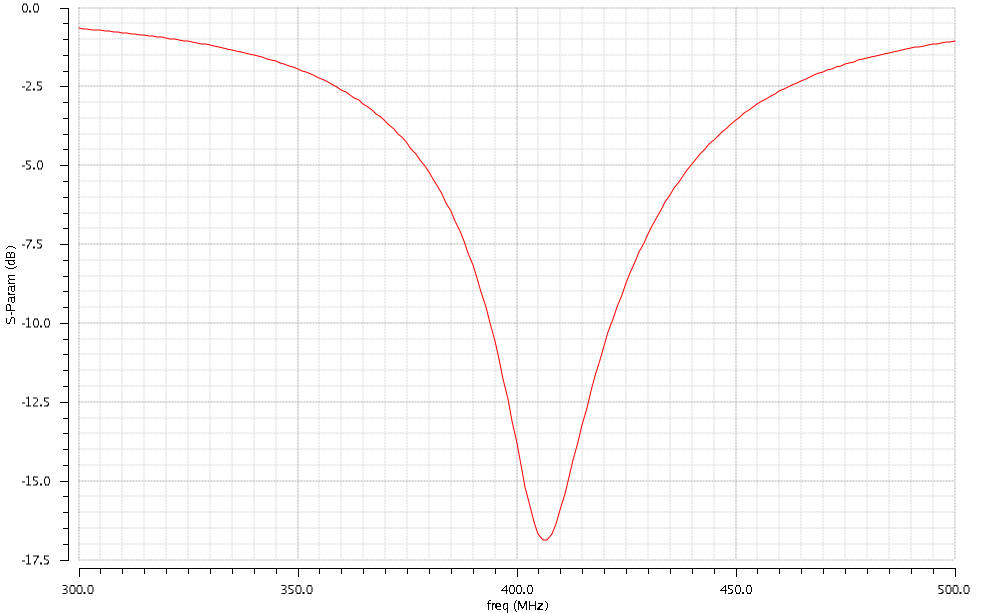
\includegraphics[width=0.5\textwidth]{figures/s11.png}
    \caption{}
    \label{fig:s11}
\end{figure}

%s22
\begin{figure}[h]
   \centering
    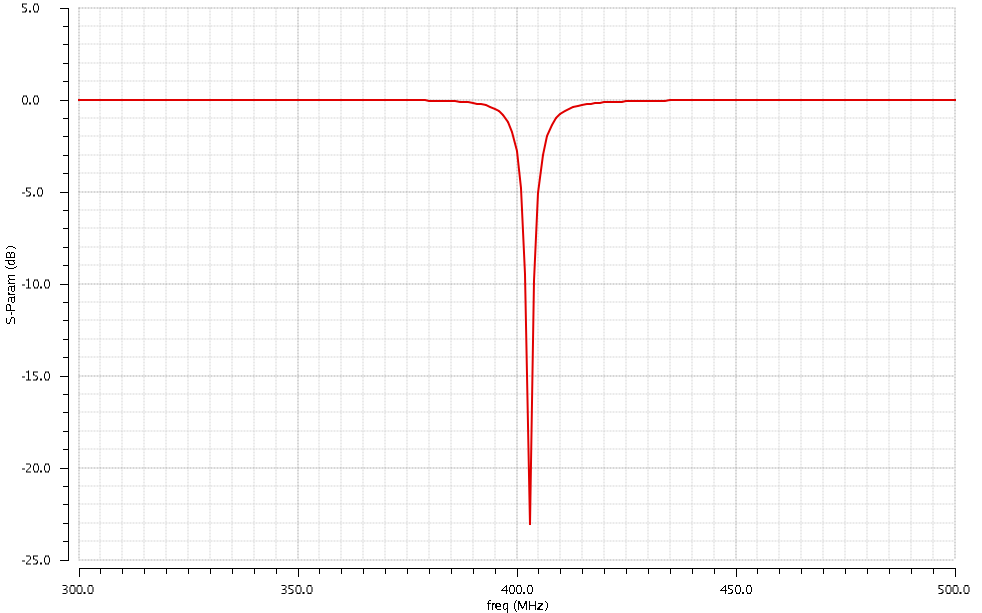
\includegraphics[width=0.5\textwidth]{figures/s22.png}
    \caption{}
    \label{fig:s22}
\end{figure}

%s21
\begin{figure}[h]
   \centering
    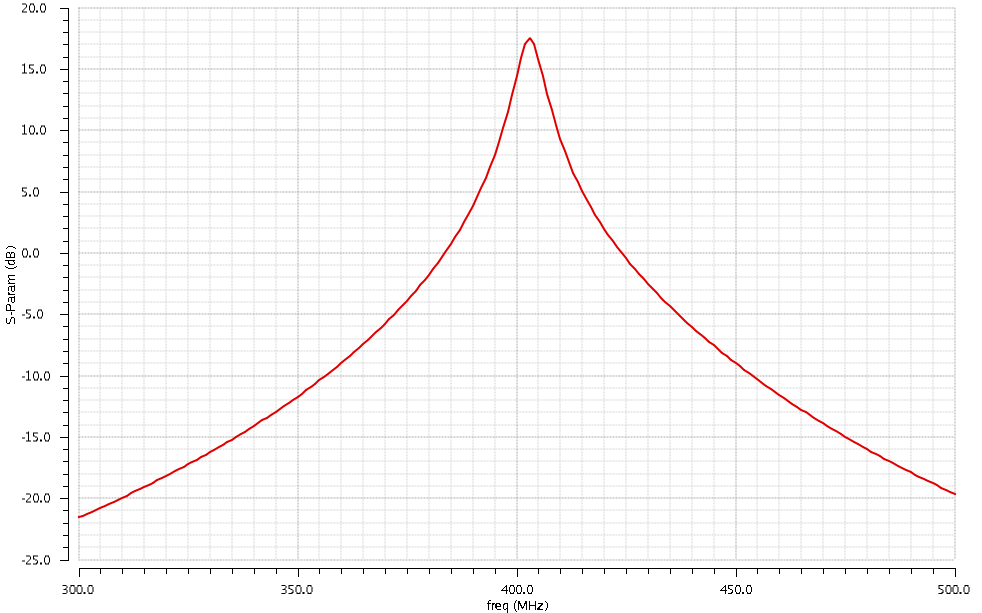
\includegraphics[width=0.5\textwidth]{figures/s21.png}
    \caption{}
    \label{fig:s21}
\end{figure}

%1dbcompression
\begin{figure}[h]
   \centering
    \includegraphics[width=0.5\textwidth]{figures/1db.png}
    \caption{}
    \label{fig:1db}
\end{figure}

%IIP3
\begin{figure}[h]
   \centering
    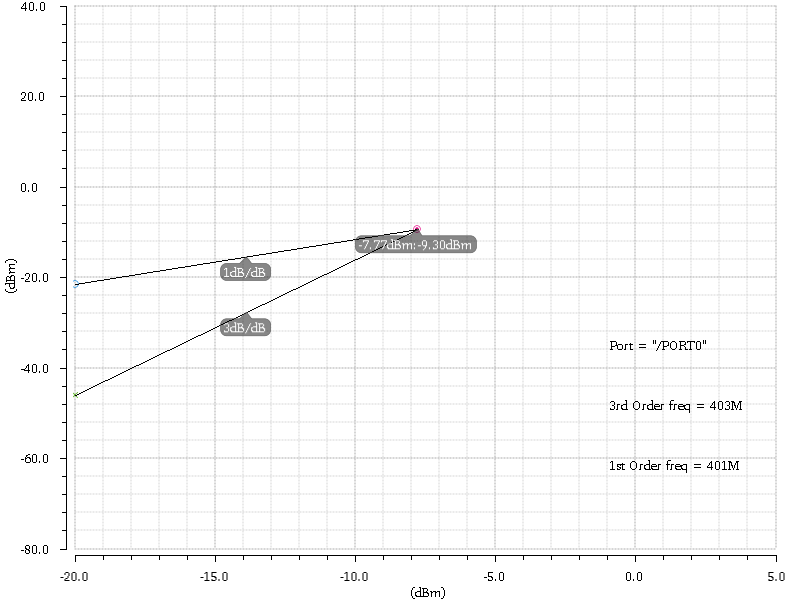
\includegraphics[width=0.5\textwidth]{figures/lnaiip3.png}
    \caption{}
    \label{fig:lnaiip3}
\end{figure}

%noise
\begin{figure}[h]
   \centering
    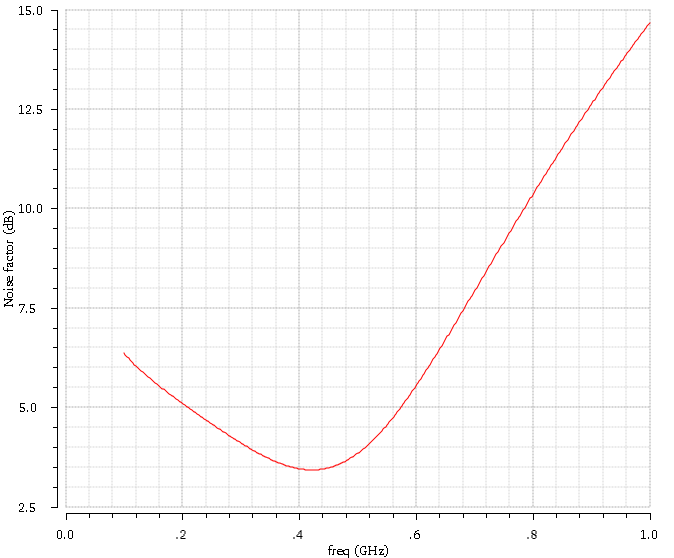
\includegraphics[width=0.5\textwidth]{figures/lnanoise.png}
    \caption{ }
    \label{fig:lnanoise}
\end{figure}

%min noise
\begin{figure}[h]
   \centering
    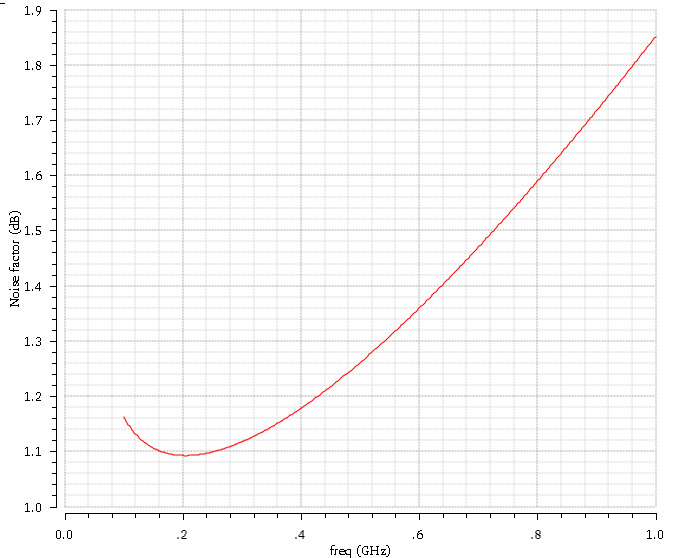
\includegraphics[width=0.5\textwidth]{figures/lnanoisemin.png}
    \caption{}
    \label{fig:lnanoisemin}
\end{figure}

\subsection{Voltage Controlled Oscillator}
Fig.2 shows the simulated output transients of the proposed VCO; the VCO provides two differential outputs with the same peak-peak value of 305 mV. The oscillation frequency can also be calculated from the period of sinusoidal waveform, which is 400 MHz. The phase noise is shown in Fig.3 and it is -119 dBc/Hz at 1MHz offset from the center frequency of 400 MHz. Fig.4 plots the simulated tuning curve by varying the controllable voltage. As the tuning voltage sweeps from -0.5 V to 1 V, the oscillation frequency changes from 393 MHz to 400 MHz, indicating a tunable range of 6 MHz. The VCO’s power consumption, which is a critical consideration in Medradio application, is 0.2 mW.